\message{ !name(06-backprop.tex)}\documentclass{beamer}
\usepackage{tikz}
\usepackage[all]{xy}
\usepackage{amsmath,amssymb}
\usepackage{hyperref}
\usepackage{graphicx}
\usepackage{algorithmic}
\usepackage{multirow}
 
\DeclareMathOperator*{\argmin}{arg\,min}
\DeclareMathOperator*{\Lik}{Lik}
\DeclareMathOperator*{\PoissonLoss}{PoissonLoss}
\DeclareMathOperator*{\Peaks}{Peaks}
\DeclareMathOperator*{\Segments}{Segments}
\DeclareMathOperator*{\argmax}{arg\,max}
\DeclareMathOperator*{\maximize}{maximize}
\DeclareMathOperator*{\minimize}{minimize}
\newcommand{\sign}{\operatorname{sign}}
\newcommand{\RR}{\mathbb R}
\newcommand{\ZZ}{\mathbb Z}
\newcommand{\NN}{\mathbb N}
\newcommand{\z}{$z = 2, 4, 3, 5, 1$} 

\newcommand{\algo}[1]{\textcolor{#1}{#1}}
\definecolor{PDPA}{HTML}{66C2A5}
\definecolor{CDPA}{HTML}{FC8D62}
\definecolor{GPDPA}{HTML}{4D4D4D}

% Set transparency of non-highlighted sections in the table of
% contents slide.
\setbeamertemplate{section in toc shaded}[default][100]
\AtBeginSection[]
{
  \setbeamercolor{section in toc}{fg=red} 
  \setbeamercolor{section in toc shaded}{fg=black} 
  \begin{frame}
    \tableofcontents[currentsection]
  \end{frame}
}

\begin{document}

\message{ !name(06-backprop.tex) !offset(638) }
\section{Multi-class classification}

\begin{frame}
  \frametitle{Review of logistic loss for binary classification}
  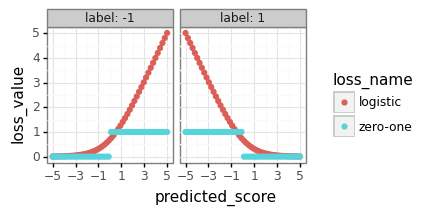
\includegraphics[width=0.7\textwidth]{2022-02-15-simplex-binary-loss-scores.png}

  \begin{itemize}
  \item For binary classification we have labels
    $\underline y\in\{-1,1\}$ (underline for label coded as -1 or 1).
  \item Let $f(x)=\hat y\in\mathbb R$ be the predicted score (output
    of neural network).
  \item The logistic loss is $\ell(\hat y, \underline y) = \log[1+\exp(\hat y \underline y)]$.
  \item Minimizing the logistic loss is equivalent to maximizing the
    binomial likelihood (sometimes called Bernoulli, special case when
    there is 1 trial), ex: flipping coins or rolling dice.
  \item The binomial distribution (two classes) is a special case of
    the multinomial distribution (two or more classes).
  \end{itemize}

\end{frame}

\begin{frame}
  \frametitle{Probabilistic interpretation of logistic loss}
  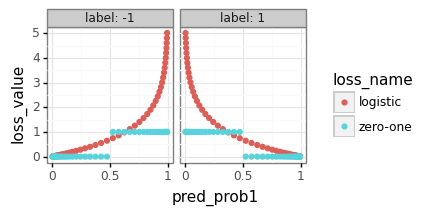
\includegraphics[width=0.7\textwidth]{2022-02-15-simplex-binary-loss-prob.png}

  \begin{itemize}
  \item Let $y\in\{0,1\}$ be the binary class label (non-negative integer).
  \item Let $\hat p_1=1/(1+\exp(-\hat y))\in (0,1)$ be the predicted probability
    of class 1 (positive), output by the neural network.
  \item Then $\hat p_0 = 1-\hat p_1$ is the predicted probability of
    negative class.
  \item Then the logistic loss is the negative log
    probability/likelihood of the label class,
    \begin{eqnarray*}
      \ell(\hat y, y) 
      % &=& -\log[\hat p_1 I(y=1) + \hat p_0 I(y=0)] \\
        &=& \begin{cases}
              -\log[\hat p_1] & \text{ if label is positive, } y=1 \\
              -\log[\hat p_0] & \text{ if label is negative, } y=0
            \end{cases}\\
        &=& -\log[\hat p_y].
    \end{eqnarray*}
  \end{itemize}

\end{frame}

\begin{frame}
  \frametitle{Multi-class loss and softmax function}

  \begin{itemize}
  \item We assume there are $K\geq 2$ classes of labels,
    $y\in\{0,1, \dots, K-1\}$.
  \item The neural network can output a probability for each
    class, $\hat p = [\hat p_0,\hat p_1,\dots,\hat p_{K-1}]$, with
    $\hat p_j\in[0,1]$ and $\sum_j \hat p_j=1$.
  \item The loss function to minimize via gradient descent is the
    negative log likelihood of the label class, $\ell[\hat p,y] = -\log \hat p_y.$
  \item The neural network last linear layer outputs $K$
    units/features (real numbers from matrix multiplication, possibly
    negative), one for each class:
    $\hat y_0,\hat y_1,\dots, \hat y_{K-1}\in\mathbb R$.
  \item To convert to a vector of probability values, we use the
    softmax function, 
$$ \hat p=\text{softmax}(\hat y_0, \dots, \hat y_{K-1}) = 
\left[ \frac{\exp\hat y_0}{\sum_{j=0}^{K-1} \exp\hat y_j}, \dots,
\frac{\exp\hat y_{K-1}}{\sum_{j=0}^{K-1} \exp\hat y_j}\right].
$$
\item (exp converts to positive, division normalizes to one)
  \end{itemize}
\end{frame}

\begin{frame}
  \frametitle{Visualization of loss functions for 3 class problem}
  
  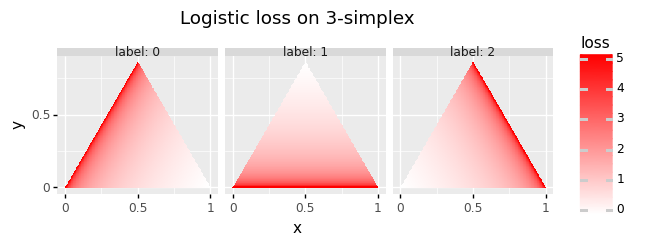
\includegraphics[width=0.7\textwidth]{2022-02-15-simplex-multi-logistic}

  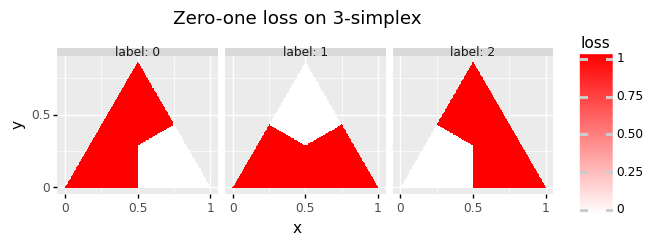
\includegraphics[width=0.7\textwidth]{2022-02-15-simplex-multi-zero-one}

  \begin{itemize}
  \item Each point in 3-simplex is a probability triple
    $(p_0,p_1,p_2)$.
  \item Corners: max prob. for one class (1,0,0)
    or (0,1,0) or (0,0,1).
  \item Midpoint when classes have equal probability
    $(1/3, 1/3, 1/3)$.
  \item Zero-one loss =0 when label class most probable.
  \end{itemize}
\end{frame}

\begin{frame}
  \frametitle{Note about over-parameterization}

  \begin{itemize}
  \item A neural network for $K$ classes which outputs $K$ features is
    actually over-parameterized (but easy to code).
  \item For $K$ classes, we only need $K-1$ outputs (fewer parameters
    in last weight matrix, more computationally efficient).
  \item For example, binary classification, $K=2$, we only need 1
    output (higher values mean more likely positive class).
  \item For example, $K=3$ classes, $f(x)=[\hat p_1,\hat p_2]$ only
    needs parameters for two outputs, and the third class probability
    can be derived from the other two, $\hat p_0=1-\hat p_1-\hat p_2$.
  \end{itemize}
\end{frame}

\begin{frame}
  \frametitle{Predicted probability and loss}

  \begin{itemize}
  \item Let $z\in\mathbb R^K$ be a vector of real-valued predictions
    (inputs to softmax), same as neural network outputs if
    over-parameterized with $K$ outputs
    $\hat y_0, \hat y_1,\dots,\hat y_{K-1}$.
  \item Otherwise if neural network only has $K-1$ outputs
    $\hat y_1,\dots,\hat y_{K-1}$ then
    $z=[0,\hat y_1,\dots,\hat y_{K-1}]$.
  \item Then the predicted probability vector is
    $\hat p=\text{softmax}(z_0,\dots,z_{K-1})$.
  \item The loss function is the negative log probability of the label
    class,
$$ 
-\log \hat p_y = -\log
\left[
\frac{
  \exp(z_y)
}{
  \sum_{j=0}^{K-1}
  \exp(z_j)
}
\right]
=
\log
\left[
\sum_{j=0}^{K-1}  \exp(z_j) 
\right]
-z_y.
$$
  \end{itemize}
  
\end{frame}

\begin{frame}
  \frametitle{Binary classification is a special case 1}
  \begin{itemize}
  \item For label $y$ and real-valued predictions $z_0,\dots,z_{K-1}$, loss is
$
\log
\left[
\sum_{j=0}^{K-1}  \exp(z_j) 
\right]
-z_y.
$
\item In binary classification, $K=2$ classes, the neural network
  outputs a single score $\hat y\in\mathbb R$, larger values mean more
  likely to be positive class.
\item Let $z=[0,\hat y]$, then $\sum_{j=0}^{K-1} \exp(z_j) = 1+\exp(\hat y)$.
\item If label is positive, $y=1$, then $z_y=\hat y$ and loss is 
$$
\log
\left[
1+\exp(\hat y)
\right]
-\hat y
=
\log\left[
\frac{1+\exp(\hat y)}{\exp(\hat y)}
\right]
=
\log[1+\exp(-\hat y)].
$$
\item If label is negative, $y=0$, then $z_y=0$ and loss is
$
\log
\left[
1+\exp(\hat y)
\right].
$
\item Both cases agree with our previous logistic loss formula,
  $\log[1+\exp(-\underline y \hat y)]$, with $\underline y\in\{-1,1\}$.
\end{itemize}
\end{frame}

\begin{frame}
  \frametitle{Note about numerical stability}
  \begin{itemize}
  \item For label $y$ and real-valued predictions $z_0,\dots,z_{K-1}$, loss is
$$
\log
\left[
\sum_{j=0}^{K-1}  \exp(z_j) 
\right]
-z_y= L-z_y.
$$
\item exp may overflow to $\infty$ if $z_j$ values are too large (bad).
\item Numerical issues can be limited by using the log-sum-exp trick:
  let $M=\max_j z_j$, then
$$
L = \log
\left[
\sum_{j=0}^{K-1}  \exp(z_j) 
\right]
= 
% M - M + \log
% \left[
% \sum_{j=0}^{K-1}  \exp(z_j) 
% \right]
% = 
M+\log
\left[
\sum_{j=0}^{K-1}  \exp(z_j-M) 
\right].
$$
  \end{itemize}
\end{frame}

\begin{frame}
  \frametitle{Gradient computation}
  \begin{itemize}
  \item For label $y$ and real-valued predictions $z_0,\dots,z_{K-1}$, loss is
$
\log
\left[
\sum_{j=0}^{K-1}  \exp(z_j) 
\right]
-z_y= L-z_y.
$
\item Partial derivative with respect to prediction for class
  $k\in\{0,\dots,K-1\}$ can be written in terms of indicator function
  $I$ (1 if argument is true, otherwise 0):
$$
\frac{\partial}{\partial z_k}
\left(L-z_y\right) = 
\frac{\exp(z_k)}{\sum_{j=0}^{K-1}\exp(z_j)}
-I[y=k].
$$
\item We compute $L$ during forward pass to get loss and then use it
  again in backward pass, since $\exp(L)=\sum_{j=0}^{K-1}\exp(z_j)$,
$$
\frac{\partial}{\partial z_k}
\left(L-z_y\right) = 
\frac{\exp(z_k)}{\exp(L)}
-I[y=k]
=
\exp(z_k-L)
-I[y=k].
$$
\end{itemize}
\end{frame}

\begin{frame}
  \frametitle{Binary classification is a special case 2}
  \begin{itemize}
  \item For label $y$ and real-valued predictions $z_0,\dots,z_{K-1}$,
    partial derivative for class $k\in\{0,\dots,K-1\}$ is 
$$
\frac{\partial}{\partial z_k}
\left(L-z_y\right) = 
\frac{\exp(z_k)}{\sum_{j=0}^{K-1}\exp(z_j)}
-I[y=k].
$$
\item In binary classification, $K=2$ classes, the neural network
  outputs a single score $\hat y\in\mathbb R$, larger values mean more
  likely to be positive class.
\item Let $z=[0,\hat y]$, then $\sum_{j=0}^{K-1} \exp(z_j) = 1+\exp(\hat y)$.
\item Partial derivative with respect to predictions $\hat y$ is
$$
\frac{\partial}{\partial \hat y}
\left(L-z_y\right) 
= 
\frac{\exp(\hat y)}{1+\exp(\hat y)}
-I[y=1]
= 
\frac{1}{1+\exp(-\hat y)}
-I[y=1].
$$
\item If label is positive, $y=1$, then gradient is 
$-1/[1+\exp(\hat y)]$.
\item If label is negative, $y=0$, then gradient is
$1/[1+\exp(-\hat y)]$.
\item Both cases agree with our previous logistic loss gradient formula,
  $(-\underline y)/[1+\exp(\underline y \hat y)]$, with $\underline y\in\{-1,1\}$.
\end{itemize}
\end{frame}

\begin{frame}[fragile]
  \frametitle{Gradient example}
  \scriptsize
\begin{verbatim}
>>> def show(a):
...     return np.column_stack([np.round(a, decimals=1), batch_labels])
>>> np.row_stack([
...     show(stable_prob_mat),
...     np.repeat(np.nan, n_classes+1),
...     show(-stable_grad_mat)
... ])
array([[ 0. ,  0. ,  0. ,  0. ,  0. ,  0. ,  1. ,  0. ,  0. ,  0. ,  9. ],
       [ 0. ,  0.5,  0. ,  0. ,  0. ,  0. ,  0.5,  0. ,  0. ,  0. ,  6. ],
       [ 0. ,  0. ,  0. ,  0.1,  0. ,  0. ,  0.9,  0. ,  0. ,  0. ,  3. ],
       [ 0. ,  0. ,  0. ,  0. ,  0. ,  0. ,  1. ,  0. ,  0. ,  0. ,  6. ],
       [ 0. ,  1. ,  0. ,  0. ,  0. ,  0. ,  0. ,  0. ,  0. ,  0. ,  6. ],
       [ 0. ,  0. ,  0. ,  0. ,  0. ,  0. ,  0. ,  0. ,  1. ,  0. ,  0. ],
       [ nan,  nan,  nan,  nan,  nan,  nan,  nan,  nan,  nan,  nan,  nan],
       [-0. , -0. , -0. , -0. , -0. , -0. , -1. , -0. , -0. ,  1. ,  9. ],
       [-0. , -0.5, -0. , -0. , -0. , -0. ,  0.5, -0. , -0. , -0. ,  6. ],
       [-0. , -0. , -0. ,  0.9, -0. , -0. , -0.9, -0. , -0. , -0. ,  3. ],
       [-0. , -0. , -0. , -0. , -0. , -0. ,  0. , -0. , -0. , -0. ,  6. ],
       [-0. , -1. , -0. , -0. , -0. , -0. ,  1. , -0. , -0. , -0. ,  6. ],
       [ 1. , -0. , -0. , -0. , -0. , -0. , -0. , -0. , -1. , -0. ,  0. ]])
\end{verbatim}
\end{frame}


\message{ !name(06-backprop.tex) !offset(813) }

\end{document}